\section{IMS Overview} \label{sec:scalims-background}
%\begin{comment}
\begin{figure}[!h]
        \centering
        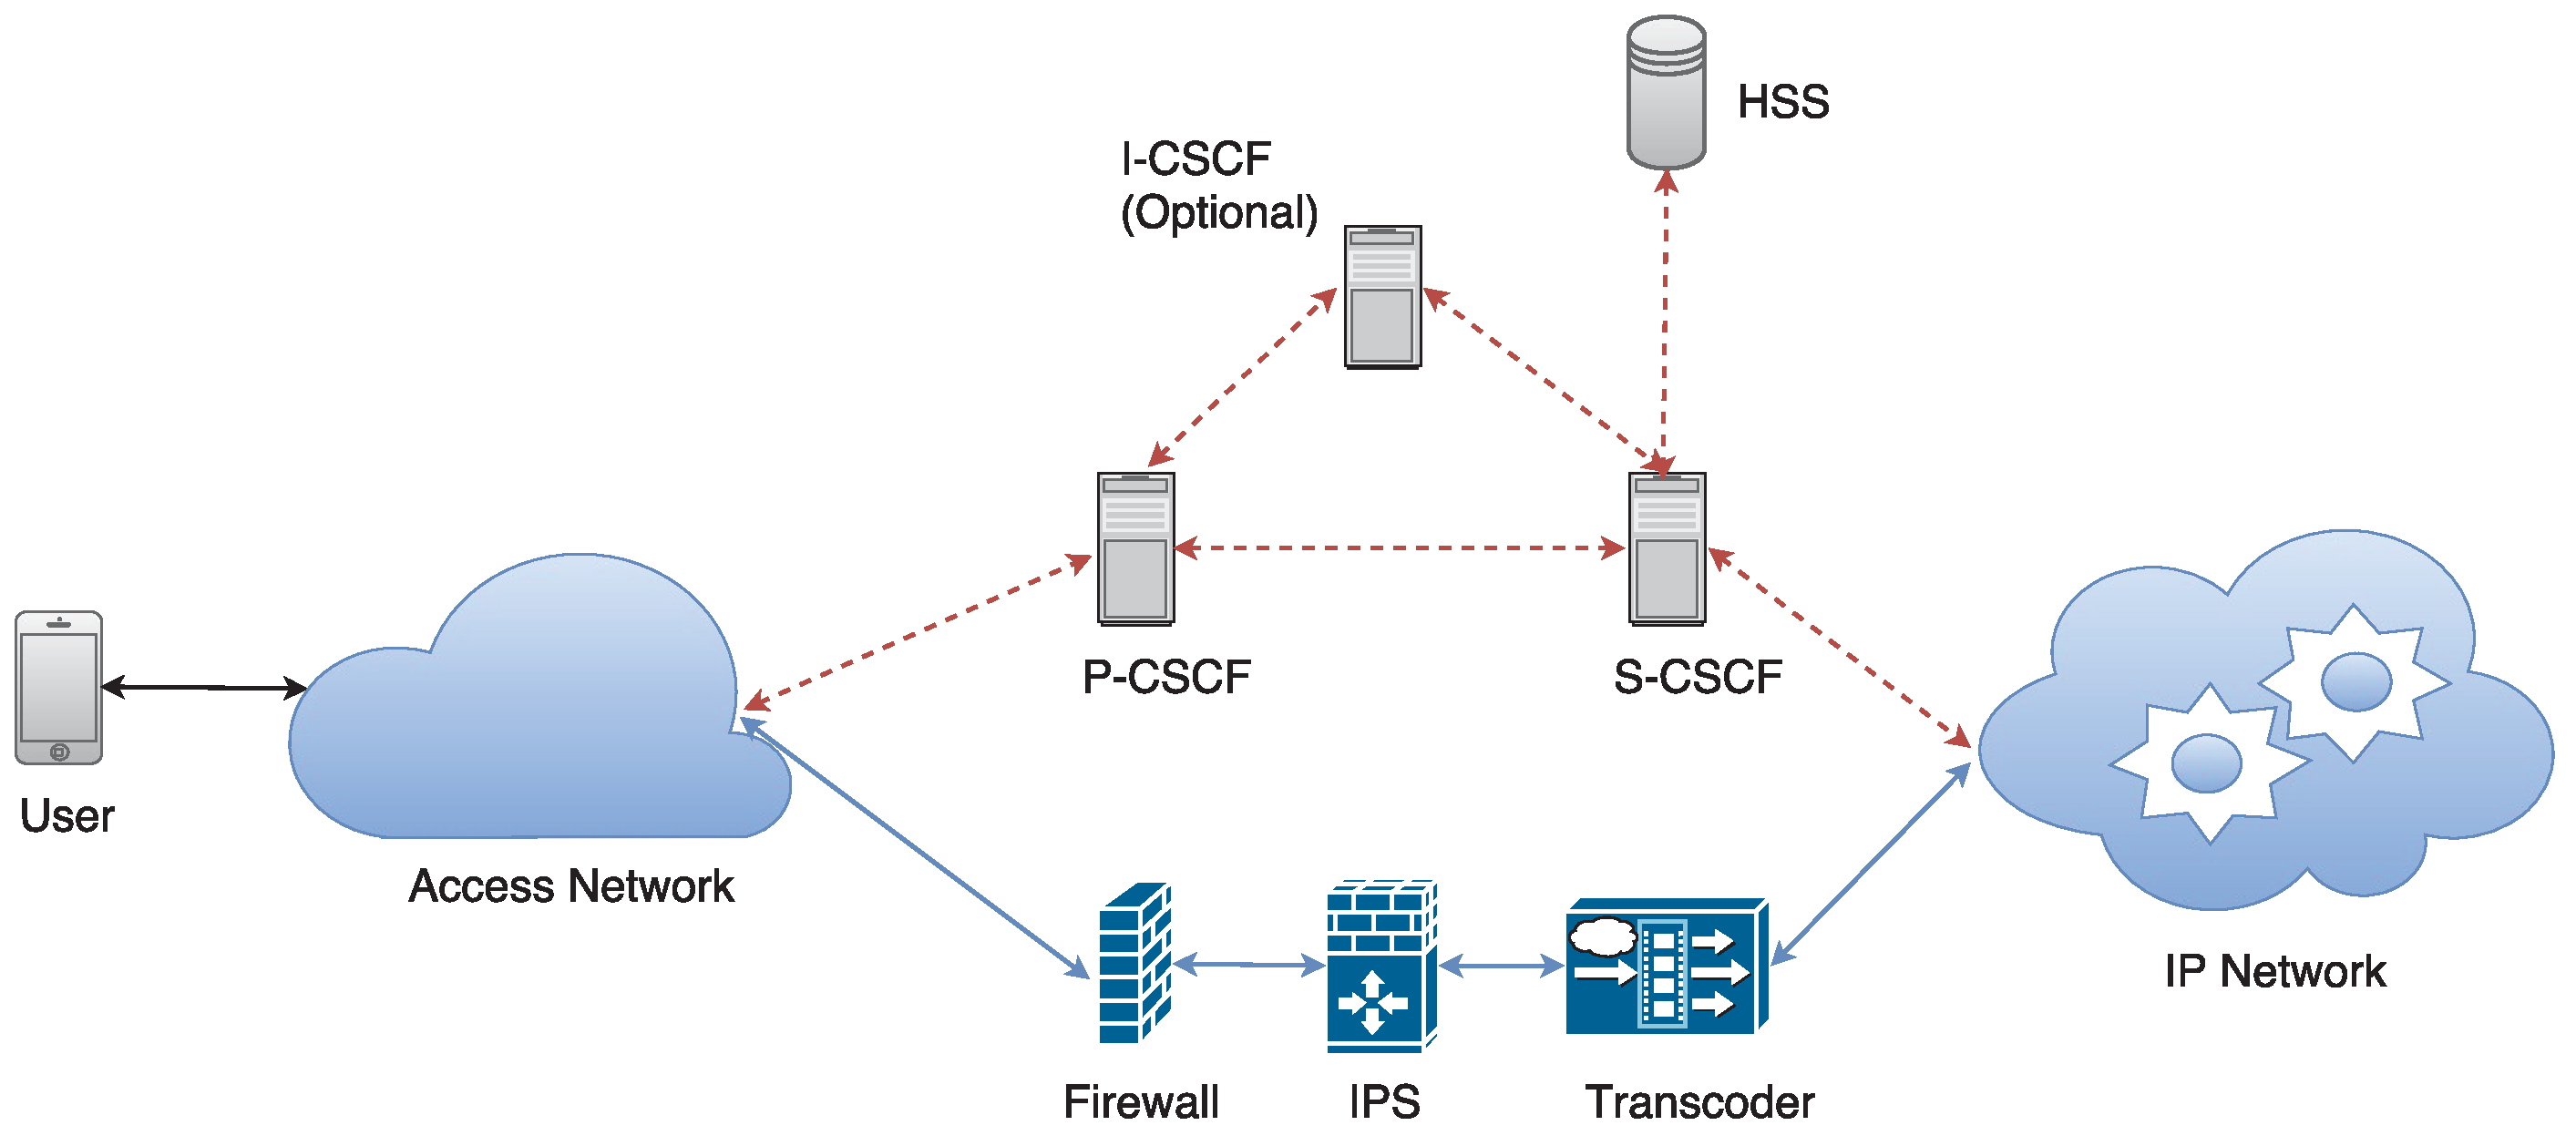
\includegraphics[width=1\columnwidth]{chap-scalims/figure/IMS_architecture.eps}
        \caption{IMS: an architectural overview}
        \label{fig:IMS_architecture}
\end{figure}
%\end{comment}

%cut for space
%old
%An IP Multimedia System (IMS) is a core part in 3G/4G telecom networks (e.g., 3GPP, 3GPP2)~\cite{umts}~\cite{lte}, responsible for delivering multimedia services (e.g., voice, video, messaging) over IP networks. IMS is a fully standardized solution for multimedia service delivery in the telecom industry~\cite{3gpp-ims}, as compared to its proprietary alternatives (e.g., Skype, Facetime). It is a complex system consisting of multiple service chains. We investigate two most important service chains as follows. An illustration is given in Fig.~\ref{fig:IMS_architecture}.
%new
An IP Multimedia Subsystem (IMS)~\cite{3gpp-ims} is a core part in 3G/4G telecom networks (e.g., 3GPP, 3GPP2)~\cite{umts}~\cite{lte}, responsible for delivering multimedia services (e.g., voice, video, messaging) over IP networks. It is a complex system consisting of multiple service chains. We investigate two most important service chains as follows. An illustration is given in Fig.~\ref{fig:IMS_architecture}.

$\triangleright$ \noindent\textbf{Control Plane (CP) Service Chain} includes three main network functions, {Proxy-CSCF (P-CSCF)}, {Interrogating-CSCF (I-CSCF)}, and {Serving-CSCF (S-CSCF)}, %collectively called Call Session Control Function (CSCF),
 which collectively handle user registration, user authentication and call setup. These network functions rely on the Session Initiation Protocol (SIP)~\cite{sip} to interoperate with users of the IMS system. Users can only contact with P-CSCF, which acts as a relay point between users and S-CSCF. Since I-CSCF acts as a middleman that forwards SIP messages between P-CSCF and S-CSCF, real-world implementation sometimes merges I-CSCF into S-CSCF as in \cite{project-clearwater} to simplify the structure of the IMS control plane service chain, making I-CSCF optional. S-CSCF %is the pivot on the control plane. It
  dispatches SIP messages to their final destinations and constantly queries an external storage server called Home Subscriber Server (HSS), which is a database that contains identities of the users. We consider the control plane service chain $\text{P-CSCF} \rightarrow \text{S-CSCF} \rightarrow \text{P-CSCF}$ in \textit{ScalIMS}. % scales the simplified control plane service chain, which has the form of $\text{P-CSCF} \rightarrow \text{S-CSCF} \rightarrow \text{P-CSCF}$.


\begin{comment}
\vspace{-3mm}
\begin{table}[!h]
        \small
        \begin{center}
        \begin{tabular}{p{0.15\linewidth}|p{0.7\linewidth}}
                %\hline
                %NF  & Description\\
                \hline
                P-CSCF & Point of attachment of a user to the IMS. Assigned to user and remains unchanged all time.\\
                \hline
                I-CSCF & Optional for security reason, forwards SIP request or response to the S-CSCF.\\
                \hline
                S-CSCF & Handles SIP message with the help of HSS, and binds the user IP address and the SIP address.\\
                \hline
        \end{tabular}
       % \caption{Network functions for the IMS control plane}
       % \label{tab:control-plane}

        \end{center}
\end{table}
\end{comment}

$\triangleright$ \noindent\textbf{Data Plane (DP) Service Chain} contains a sequence of network functions that the actual multimedia traffic between users traverses, for security (e.g., firewall, deep packet inspection, intrusion detection), connectivity (e.g., NAT, IPv4-to-IPv6 conversion), quality of service (e.g., traffic shaping, rate limiting, ToS/DSCP bit setting), and media processing (e.g., transcoding). While 3GPP has standardized the IMS control plane for interoperability reasons, the exact set of deployed network functions for the data plane varies per operator.


The two service chains collectively handle two important procedures of the IMS system, which are user registration and call setup. %User registration is performed through a SIP REGISTRATION transaction over the control plane.
To make a call, a user first registers his IP address to the IMS by initiating a SIP REGISTRATION transaction over the CP. When the registration is done, S-CSCF temporarily stores the binding between the identity of the user and the P-CSCF instance connected to the user for future calls. To setup a call between a caller and a callee, the caller initiates a SIP INVITE transaction to the IMS, specifying the identify of the callee. S-CSCF uses the binding saved during user registration to retrieve the P-CSCF instance that the callee connects to and sends the message to the P-CSCF instance, which forwards to the callee. After the callee responds, a call is successfully set up. Subsequent media flows between the caller and the callee are routed through DP service chain. When the call is finished, a SIP BYE transaction between the caller and the callee is carried out to close the call over the CP.

%A good NFV management system should effectively scales both the control and data plane service chains of the IMS system. %Since the operation of these two service chains are coupled together through SIP protocol, \textit{ScalIMS} uses a novel method based on flow tagging to effectively scale these two service chains.
